\documentclass{beamer}
\usetheme{CambridgeUS}
\usepackage{listings}
\usepackage{blkarray}
\usepackage{listings}
\usepackage{subcaption}
\usepackage{url}
\usepackage{tikz}
\usepackage{tkz-euclide} % loads  TikZ and tkz-base
%\usetkzobj{all}
\usetikzlibrary{calc,math}
\usepackage{float}
\renewcommand{\vec}[1]{\mathbf{#1}}
\usepackage[export]{adjustbox}
\usepackage[utf8]{inputenc}
\usepackage{amsmath}
\usepackage{amsfonts}
\usepackage{tikz}
\usepackage{hyperref}
\usepackage{bm}
\usetikzlibrary{automata, positioning}
\providecommand{\pr}[1]{\ensuremath{\Pr\left(#1\right)}}
\providecommand{\mbf}{\mathbf}
\providecommand{\qfunc}[1]{\ensuremath{Q\left(#1\right)}}
\providecommand{\sbrak}[1]{\ensuremath{{}\left[#1\right]}}
\providecommand{\lsbrak}[1]{\ensuremath{{}\left[#1\right.}}
\providecommand{\rsbrak}[1]{\ensuremath{{}\left.#1\right]}}
\providecommand{\brak}[1]{\ensuremath{\left(#1\right)}}
\providecommand{\lbrak}[1]{\ensuremath{\left(#1\right.}}
\providecommand{\rbrak}[1]{\ensuremath{\left.#1\right)}}
\providecommand{\cbrak}[1]{\ensuremath{\left\{#1\right\}}}
\providecommand{\lcbrak}[1]{\ensuremath{\left\{#1\right.}}
\providecommand{\rcbrak}[1]{\ensuremath{\left.#1\right\}}}
\providecommand{\abs}[1]{\vert#1\vert}
\newcommand*{\permcomb}[4][0mu]{{{}^{#3}\mkern#1#2_{#4}}}
\newcommand*{\perm}[1][-3mu]{\permcomb[#1]{P}}
\newcommand*{\comb}[1][-1mu]{\permcomb[#1]{C}}
\renewcommand{\thetable}{\arabic{table}} 
\newcounter{saveenumi}
\newcommand{\seti}{\setcounter{saveenumi}{\value{enumi}}}
\newcommand{\conti}{\setcounter{enumi}{\value{saveenumi}}}
\usepackage{amsmath}
\setbeamertemplate{caption}[numbered]{}
\DeclareUnicodeCharacter{2212}{\textendash}
\title{AI1110 Assignment 7}
\author{SADINENI ABHINAY-CS21BTECH11055}
\date{\today}
\begin{document}
	
	\begin{frame}
		\titlepage
	\end{frame}

\begin{frame}{Outline}
  \tableofcontents
\end{frame}

\section{Abstract}
	\begin{frame}{Abstract}
		\begin{itemize}
			\item 	This document contains the solution to Question of Chapter 13 (Probability) in the NCERT Class 12 Textbook.
		\end{itemize}
	\end{frame}
	
	\section{Question}
	\begin{frame}{Question}
		\begin{block}{\textbf{Probability  ex 13.5 q8.}}
			 Suppose X has a binomial distribution $B\brak{6,\frac{1}{2}}$ .Show that $X=3$ is most likely outcome.
			 \brak{hint: \pr{X=3} \text{is the max among all} \pr{x_i}, x_{i}=0,1,2,3,4,5,6}
		\end{block}
	\end{frame}
	

	\section{Theory}
	\begin{frame}{Theory}
			 \begin{block}{Binomial Distribution}
	      the binomial distribution with parameters n and p is the discrete probability distribution of the number of successes in a sequence of n independent experiments, each asking a yes–no question, and each with its own Boolean-valued outcome: success (with probability p) or failure (with probability $q = 1 − p$)
		\end{block}	   
			      The Expression is given by:
\begin{align}
\sum_{i=0}^{n}\pr{X = i} =  \sum_{i=0}^{n} \comb{n}{i}(\text{p})^i\left(1-\text{p}\right)^{n-i}
\\
\pr{X = i} =\comb{n}{i}(\text{p})^i\left(1-\text{p}\right)^{n-i}
	      \end{align}
	\end{frame}
	
	\section{Generalized problem}
	\begin{frame}{Generalized problem}
	\begin{block}{}
	 Suppose X has a binomial distribution $B\brak{n,p}$ .Find the most likely outcome.
	\end{block}
	\end{frame}
	\section{Solution}	
	\begin{frame}{Solution}
		Given X has binomial distribution B\brak{n,p}
		as we know
		\begin{align}
		\pr{X = i} =\comb{n}{i}(\text{p})^i\left(1-\text{p}\right)^{n-i}
		\end{align}
		Now to find maximum probability the following conditions
		\begin{align}
		\frac{\pr{X=k}}{\pr{X=\brak{k+1}}}\ge 1 \label{eq:eq4}
		\\
		 \frac{\pr{X=k}}{\pr{X=\brak{k-1}}} \ge 1 \label{eq:eq5}
		\end{align}
	\end{frame}

	\begin{frame}{}
	Solving equation \eqref{eq:eq4}
	\begin{align} 
	    \frac{\pr{X=k}}{\pr{X=\brak{k-1}}} &=\frac{\comb{n}{k}}{\comb{n}{k-1}}.\frac{p^{k}\brak{1-p}^{n-k}}{p^{k-1}\brak{1-p}^{n+1-k}}=\frac{n+1-k}{k}.\frac{p}{1-p} 
	    \end{align}
	    \begin{align}
	  &\implies \frac{n+1-k}{k}.\frac{p}{1-p} \ge 1\\
	  &\implies k \le \brak{n+1}p
	    \end{align}
	    Solving equation \eqref{eq:eq5}
	\begin{align} 
	    \frac{\pr{X=k}}{\pr{X=\brak{k+1}}} &=\frac{\comb{n}{k}}{\comb{n}{k+1}}.\frac{p^{k}\brak{1-p}^{n-k}}{p^{k-1}\brak{1-p}^{n-1-k}}=\frac{k+1}{n-k}.\frac{1-p}{p} 
	    \end{align}
	    \begin{align}
	  &\implies \frac{k+1}{n-k}.\frac{1-p}{p} \ge 1\\
	  &\implies k \ge \brak{n+1}p-1
	    \end{align}
	    \end{frame}
\section{Result}
\begin{frame}{Result}
\begin{block}{Result}
Combining Results from two conditions 
\begin{align}
\brak{n+1}p-1 \le k \le \brak{n+1}p
\end{align}
 k must be a integer in between these two values ,X=k is the most likely outcome\\
 \textbf{Note:}
 if \brak{n+1}p is integer then k can have both values ie. \brak{n+1}p-1 and \brak{n+1}p

\end{block}
\end{frame}

\section{Answer}
\begin{frame}{Answer}
For this given question ,$n=6,p=\frac{1}{2}$ then 
\begin{align}
 \brak{n+1}p =3.5
  \\
 \implies 2.5 \le k \le 3.5 
\end{align}
since k is a integer the value of k is 3 \\
$\therefore X=3$  is the most likely outcome.
\end{frame}
\section{PMF}
\begin{frame}{PMF}
\begin{figure}[!ht]
		\centering
			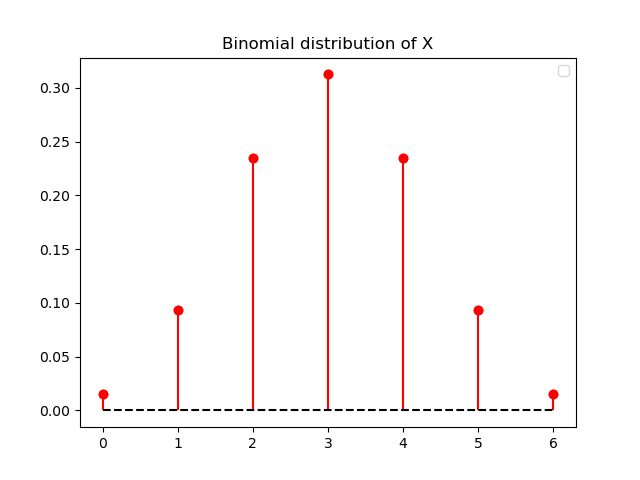
\includegraphics[width=\textwidth,height=5.5cm,keepaspectratio]{figs/binomial1.png}
		\caption{PMF}
		\label{Fig 0:}
	\end{figure}
\end{frame}
\end{document}
